\chapter{Knuth--Morris--Pratt e la funzione \texorpdfstring{$Z$}{Z}}
\label{cap:kmp-z}

\scan{3}
Fissiamo una volta per tutte le notazioni. $P$ è il \emph{pattern} e $T$ il
\emph{testo}, entrambi stringhe sull'alfabeto $\alfa$; poniamo $n=\abs{P}$ e
$m=\abs{T}$, con $n\le m$, e indicizziamo le stringhe a partire da~$1$, così che
$\sub{S}{i}{j}$ denoti il fattore di $S$ compreso fra le posizioni $i$ e $j$
estremi inclusi. Il problema dell'\emph{exact string matching} chiede di trovare
tutte le occorrenze di $P$ in $T$.

\section{Il problema e i suoi due limiti}

I due termini del confronto sono
\[
  \underbrace{\Oh(n\cdot m)}_{\text{\emph{upper bound}: l'algoritmo naive}}
  \qquad\text{contro}\qquad
  \underbrace{\Om(n+m)}_{\text{\emph{lower bound} del problema}} .
\]
Il primo è quadratico ed è il costo dell'algoritmo naive, che prova tutti gli
allineamenti di $P$ su $T$; il secondo è lineare e non è un limite inferiore del
naive, bensì del \emph{problema} --- l'input va comunque letto per intero. Resta
quindi aperta la domanda:

\begin{domanda}\label{dom:subquadratico}
  Esiste un algoritmo \underline{sub}-quadratico per l'exact string matching?
\end{domanda}

\noindent Il bersaglio è il lower bound stesso, cioè un algoritmo che lavori in
tempo
\[
  \Th(n+m),
\]
ed è esattamente ciò che Knuth--Morris--Pratt riesce a ottenere.

\section{L'idea di Knuth--Morris--Pratt}

L'idea è di non buttare via l'informazione raccolta dai confronti già eseguiti.
Supponiamo di aver allineato $P$ su $T$, di aver riconosciuto correttamente il
prefisso $\pre{P}{i}$ e di trovare un mismatch al carattere successivo: il testo
presenta un carattere $y$, il pattern presenta $x=P[i+1]$, e $x\neq y$.

Il tratto già verificato è noto \emph{a priori} --- è un prefisso di $P$,
indipendente da $T$ --- e quindi tutta l'informazione riutilizzabile può essere
ricavata dal solo pattern.

Sia $\alpha$ il più lungo \emph{prefisso-suffisso} proprio di $\pre{P}{i}$, cioè
la più lunga stringa che ne sia simultaneamente prefisso proprio e suffisso
proprio. Poiché $\alpha$ compare sia in testa a $P$ sia in coda al tratto già
riconosciuto, posso far scivolare il pattern verso destra finché il suo prefisso
$\alpha$ non si sovrappone all'occorrenza di $\alpha$ che nel testo termina
appena prima del mismatch: lo spostamento è di $i-\abs{\alpha}$ posizioni e il
confronto riprende dalla \emph{stessa} posizione del testo, ora contro
$P[\abs{\alpha}+1]$. In particolare l'indice sul testo non torna mai indietro.

\begin{figure}[H]
  \centering
  % kmp-shift -- regola di spostamento di KMP (quaderno, pag. 3).
% Tre barre sovrapposte: il testo T, il pattern P nell'allineamento corrente,
% il pattern P dopo lo scorrimento di i-|alpha| posizioni.
% Proporzioni prese dal quaderno: i = 5 unita', |alpha| = 3, spostamento = 2.
% Le due barre di P hanno la stessa lunghezza (11 unita'): e' la stessa stringa.
\begin{tikzpicture}[
    x=0.52cm, y=1cm,
    font=\footnotesize,
    >={Stealth[length=4pt,width=3pt]},
    barra/.style={line width=0.7pt},
    sep/.style={line width=0.5pt},
    guida/.style={gray!60!black, line width=0.5pt},
  ]

  % ===== colonna del mismatch (attraversa tutte e tre le righe) =========
  \draw[guida] (6,-0.45) -- (6,2.62);
  \draw[guida] (7,-0.45) -- (7,2.62);

  % ===== RIGA 1 : il testo T ===========================================
  \draw[barra] (0,2.05) rectangle (20,2.50);
  % porzione gia' scandita / non specificata
  \draw[guida] plot[domain=0.45:2.55,samples=50,smooth]
        ({\x},{2.275+0.075*sin(\x*360)});
  \draw[sep] (3,2.05) -- (3,2.50);
  \node at (4.5,2.275) {$\alpha$};
  \node at (6.5,2.275)  {$y$};
  \node[right,inner sep=3pt] at (20,2.275) {$T$};
  % punto di confronto corrente sul testo
  \draw[->,line width=0.6pt] (6.5,3.12) -- (6.5,2.68);

  % ===== mismatch ======================================================
  \node[fill=white,inner sep=1.5pt] at (6.5,1.725) {$\neq$};

  % ===== RIGA 2 : il pattern P nell'allineamento corrente ===============
  \draw[barra] (1,0.95) rectangle (12,1.40);
  % la porzione di P che lo scorrimento scarta (lunga i-|alpha|), tratteggiata
  \begin{scope}
    \clip (1,0.95) rectangle (3,1.40);
    \foreach \i in {-2,...,13}{%
      \draw[guida,line width=0.4pt]
        ({1+\i*0.30},0.90) -- ({1+\i*0.30+0.42},1.45);
    }
  \end{scope}
  \draw[sep] (3,0.95) -- (3,1.40);
  \node at (4.5,1.175) {$\alpha$};
  \node at (6.5,1.175)  {$x$};
  \node[right,inner sep=3pt] at (12,1.175) {$P$};

  % ===== RIGA 3 : il pattern P dopo lo spostamento ======================
  \draw[barra] (3,-0.35) rectangle (14,0.10);
  \node at (4.5,-0.125) {$\alpha$};
  \node at (6.5,-0.125)  {$y$};
  \node[right,inner sep=3pt] at (14,-0.125) {$P$};
  % il confronto riprende dalla stessa posizione del testo
  \draw[->,line width=0.6pt] (6.5,-1.00) -- (6.5,-0.53);

  % ===== annotazioni dello spostamento =================================
  % il prefisso alpha di P: lungo |alpha|, oltrepassa la zona tratteggiata ...
  \draw[guida,->] (1.05,0.78) to[bend right=18] (3.95,0.78);
  \draw[guida,->] (2.00,-0.02) -- (2.00,0.55);
  \node[right,inner sep=1pt] at (2.10,-0.02) {$\alpha$};
  % ... e scivola di i-|alpha| fino a sovrapporsi all'occorrenza di alpha in T
  \draw[guida,dashed,->] (1.00,-0.58) to[out=-35,in=205] (2.92,-0.30);
  % dopo lo shift il tratto alpha e' gia' verificato
  \draw[guida,->] (3.10,-0.58) to[bend right=15] (5.90,-0.58);

\end{tikzpicture}

  \caption{Regola di spostamento di KMP. Dopo aver riconosciuto $\pre{P}{i}$ il
  confronto fallisce fra il carattere $y$ del testo e $x=P[i+1]$: il pattern
  scivola di $i-\abs{\alpha}$ posizioni, fino a sovrapporre il proprio prefisso
  $\alpha$ all'occorrenza di $\alpha$ che in $T$ termina appena prima del
  mismatch. Mi sposto cioè in base al più lungo prefisso-suffisso.}
  \label{fig:kmp-shift}
\end{figure}

\paragraph{Schema dell'algoritmo.}
\begin{enumerate}
  \item \emph{Pre-processing del pattern} (che di solito è molto più piccolo del
    testo), che mi consenta, per ogni prefisso $\pre{P}{i}$, di determinare il più
    lungo prefisso-suffisso proprio, cioè
    \[
      \max\bigl\{\, k \;\bigm|\; 0\le k<i,\ \pre{P}{k} = \sub{P}{i-k+1}{i} \,\bigr\}.
    \]
    (\emph{Come farlo?} È la domanda a cui risponde la sezione seguente.)
  \item Uso il pre-processing del punto~1 per eseguire una scansione di $T$ in
    cui, ad ogni passo, posso
    \begin{itemize}
      \item o avanzare il punto di confronto,
      \item oppure avanzare il pattern.
    \end{itemize}
\end{enumerate}

\noindent Poiché ad ogni passo almeno una delle due quantità avanza, e nessuna
delle due può superare la lunghezza del testo, il numero totale di passi è
lineare e il costo complessivo è
\[
  \Th(n+m).
\]

\begin{osservazione}
  È più efficiente, per quanto possa sembrare contro\-intuitivo, preprocessare
  il \emph{testo} piuttosto che il pattern: così il tempo di ricerca di pattern
  diversi sullo stesso testo è proporzionale alla lunghezza del pattern, e non a
  quella del testo. È l'idea che sta dietro ai suffix tree e ai suffix array.
\end{osservazione}

\section{Il pre-processing del pattern: i valori
  \texorpdfstring{$\spv{i}$}{sp\_i}}
\label{sec:kmp-preprocessing}

\scan{4}
Il pre-processing di $P$ consiste nel calcolare, per ogni prefisso di $P$, il più
lungo $\alpha$ che ne sia contemporaneamente prefisso e suffisso \emph{proprio}.
Conviene enunciarlo per una stringa generica $S$ --- che nell'applicazione a KMP
sarà il pattern, cosicché $\abs{S}=n$ --- scrivendo $S_i \defeq \pre{S}{i}$ per
il suo prefisso $i$-esimo.

\begin{definizione}[Prefisso-suffisso massimo]\label{def:sp-i}
  Sia $S$ una stringa e sia $1\le i\le\abs{S}$. Poniamo
  \[
    \spv{i}(S) \defeq \max\set{\,k \;:\; 0\le k<i,\ \pre{S}{k}=\sub{S}{i-k+1}{i}\,} ,
  \]
  cioè $\spv{i}(S)$ è la lunghezza del massimo prefisso \emph{proprio} di $S_i$
  che ne sia anche suffisso; tale prefisso-suffisso si dice anche \emph{bordo}
  di $S_i$. Il vincolo $k<i$ è essenziale: senza di esso ogni
  prefisso sarebbe banalmente prefisso-suffisso di sé stesso e si avrebbe
  $\spv{i}(S)=i$. Il massimo è sempre ben definito perché $k=0$ (il bordo vuoto
  $\vuota$) soddisfa la condizione; in particolare $\spv{1}(S)=0$.
\end{definizione}

\begin{figure}[H]
  \centering
  % kmp-alfa-S -- il massimo prefisso-suffisso alpha del prefisso S_i (pag. 4).
% alpha compare una volta in testa a S e una volta in coda a S_i, e |alpha|=sp_i(S).
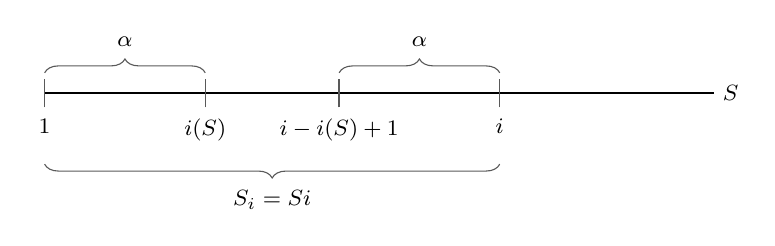
\begin{tikzpicture}[
    x=0.85cm, y=1cm,
    font=\footnotesize,
    linea/.style={line width=0.8pt},
    tacca/.style={gray!70!black, line width=0.5pt},
    graffa/.style={decorate, decoration={brace, amplitude=5pt}, gray!70!black},
  ]

  % --- la stringa S -----------------------------------------------------
  \draw[linea] (0,0) -- (10,0);
  \node[right,inner sep=3pt] at (10,0) {$S$};

  % --- confini fra caratteri --------------------------------------------
  \foreach \x in {0,2.4,4.4,6.8}{\draw[tacca] (\x,-0.18) -- (\x,0.18);}

  % --- le due occorrenze di alpha, della stessa lunghezza ---------------
  \draw[graffa] (0,0.26) -- (2.4,0.26)
        node[midway,above=6pt,black] {$\alpha$};
  \draw[graffa] (4.4,0.26) -- (6.8,0.26)
        node[midway,above=6pt,black] {$\alpha$};

  % --- posizioni ---------------------------------------------------------
  \node[below,inner sep=4pt] at (0,-0.18)   {$1$};
  \node[below,inner sep=4pt] at (2.4,-0.18) {$\spv{i}(S)$};
  \node[below,inner sep=4pt] at (4.4,-0.18) {$i-\spv{i}(S)+1$};
  \node[below,inner sep=4pt] at (6.8,-0.18) {$i$};

  % --- il prefisso S_i ---------------------------------------------------
  \draw[graffa,decoration={mirror}] (0,-0.90) -- (6.8,-0.90)
        node[midway,below=6pt,black] {$S_i = \pre{S}{i}$};

\end{tikzpicture}

  \caption{Per ogni prefisso $S_i=\pre{S}{i}$ si cerca il massimo $\alpha$ che ne
  sia al tempo stesso prefisso e suffisso: $\alpha$ compare una volta in testa a
  $S$ e una volta in coda a $S_i$, terminando in posizione $i$, e
  $\abs{\alpha}=\spv{i}(S)$.}
  \label{fig:kmp-alfa-S}
\end{figure}

\begin{osservazione}
  Il pre-processing prende tempo \emph{lineare}. È l'affermazione che ci
  accingiamo a giustificare, e non è affatto ovvia.
\end{osservazione}

\noindent Per calcolare $\spv{i}(S)$ ci sono due casi. Posto $k=\spv{i-1}(S)$ e
$\alpha=\pre{S}{k}$:
\begin{enumerate}
  \item (\emph{caso base}) se $S[i]=S[k+1]$ posso estendere $\alpha$ di un
    carattere, e
    \[
      \spv{i}(S) \;=\; \spv{i-1}(S)+1 ;
    \]
  \item altrimenti $\spv{i}(S)$ si ottiene ricorsivamente: il candidato
    successivo è $\beta$, il massimo bordo di $\alpha$, cioè
    $\abs{\beta}=\spv{k}(S)$, e si ripete il confronto fra $S[i]$ e
    $S[\abs{\beta}+1]$. Il procedimento si itera lungo la catena dei bordi
    $\alpha,\beta,\dots$ finché un carattere coincide con $S[i]$, e allora si
    ricade nel caso~1, oppure finché la catena si esaurisce nella stringa vuota:
    in tal caso $\spv{i}(S)=1$ se $S[i]=S[1]$, e $\spv{i}(S)=0$ altrimenti.
\end{enumerate}

\begin{figure}[H]
  \centering
  % kmp-bordo-del-bordo -- il passo ricorsivo del pre-processing (pag. 4).
% alpha = massimo bordo di S_{i-1} (|alpha|=k=sp_{i-1}(S)),
% beta  = massimo bordo di alpha. Qui S[i]=a diverso da b=S[k+1]:
% alpha non si estende e si ricade su beta.
\begin{tikzpicture}[
    x=0.80cm, y=1cm,
    font=\footnotesize,
    >={Stealth[length=4pt,width=3pt]},
    linea/.style={line width=0.8pt},
    tacca/.style={gray!70!black, line width=0.5pt},
    segm/.style={line width=0.6pt},
  ]

  % --- la stringa S ------------------------------------------------------
  \draw[linea] (0,0) -- (12.6,0);
  \node[right,inner sep=3pt] at (12.6,0) {$S$};
  \draw[tacca] (0,-0.16) -- (0,0.16);

  % --- le due celle di un carattere ---------------------------------------
  % b = S[k+1] segue la copia-prefisso di alpha
  \draw[segm] (4,0) rectangle (5,0.42);
  \node at (4.5,0.21) {$b$};
  % a = S[i] segue la copia-suffisso di alpha
  \draw[segm] (10,0) rectangle (11,0.42);
  \node at (10.5,0.21) {$a$};

  % --- livello 1 : le due occorrenze di alpha ------------------------------
  \foreach \s/\e in {0/4, 6/10}{%
    \draw[segm] (\s,0.62) -- (\e,0.62);
    \draw[segm] (\s,0.52) -- (\s,0.72);
    \draw[segm] (\e,0.52) -- (\e,0.72);
  }
  \node[above,inner sep=2pt] at (3.0,0.66) {$\alpha$};
  \node[above,inner sep=2pt] at (7.0,0.66) {$\alpha$};

  % --- livello 2 : beta, bordo di alpha ------------------------------------
  % beta e' prefisso di alpha (copia sinistra) e suffisso di alpha (copia destra)
  \foreach \s/\e in {0/2, 8/10}{%
    \draw[segm] (\s,1.28) -- (\e,1.28);
    \draw[segm] (\s,1.18) -- (\s,1.38);
    \draw[segm] (\e,1.18) -- (\e,1.38);
  }
  \node[above,inner sep=2pt] at (1.0,1.32) {$\beta$};
  \node[above,inner sep=2pt] at (9.0,1.32) {$\beta$};

  % il confronto del passo ricorsivo riprende dal carattere S[i]
  \draw[->,line width=0.6pt] (10.5,1.10) -- (10.5,0.52);

  % --- posizioni ----------------------------------------------------------
  \foreach \x in {4,5,10,11}{\draw[tacca] (\x,-0.16) -- (\x,0);}
  \node[below,inner sep=4pt] at (3.6,-0.10)  {$k$};
  \node[below,inner sep=4pt] at (4.5,-0.10)  {$k+1$};
  \node[below,inner sep=4pt] at (9.5,-0.10)  {$i-1$};
  \node[below,inner sep=4pt] at (10.5,-0.10) {$i$};

\end{tikzpicture}

  \caption{Il passo ricorsivo: $\alpha$ è il massimo prefisso-suffisso di
  $S_{i-1}$ e $\beta$ è il massimo prefisso-suffisso di $\alpha$. Nel disegno
  $S[i]=a \ne b=S[k+1]$, quindi $\alpha$ non si estende e si ricade su $\beta$.}
  \label{fig:kmp-bordo-del-bordo}
\end{figure}

\noindent Quante chiamate ricorsive innesca il caso~2)?

\begin{osservazione}[Problema]
  Il caso~2) può innescare fino a $i$ chiamate ricorsive: per
  $i\in\set{1,\dots,n}$ l'ordine del caso pessimo farebbe concludere che il
  pre-processing è \emph{quadratico}!
\end{osservazione}

\noindent Con l'analisi ammortizzata si vede invece che la somma delle operazioni
su \emph{tutte} le chiamate ricorsive, per $i\in\set{1,\dots,n}$, è lineare.

\subsection{Analisi ammortizzata}
\label{sec:analisi-ammortizzata}

\scan{5}
Lo schema è il seguente: ogni volta che applico il caso~1) --- quello in cui il
massimo prefisso-suffisso si estende di un carattere --- se il costo effettivo è
$k$ ne \emph{alloco} $2k$. Raddoppiando l'addebito metto da parte un credito con
cui «pago» in anticipo ogni chiamata ricorsiva del caso~2) che eseguirò per
quella posizione.

\begin{osservazione}
  Detto con una funzione potenziale: sia $\Phi$ la lunghezza del bordo corrente,
  cioè il valore $\spv{i-1}(S)$ da cui la ricorsione riparte. Il caso~1) fa
  crescere $\Phi$ di $1$, mentre ogni chiamata ricorsiva del caso~2) esegue
  $\Phi \leftarrow \spv{\Phi}(S)$ e quindi la fa \emph{decrescere strettamente}.
  Poiché $\Phi\ge 0$ e il caso~1) viene applicato al più $n$ volte in tutto, il
  numero complessivo di chiamate ricorsive del caso~2) su tutti gli
  $i\in\set{1,\dots,n}$ è a sua volta al più $n$: il credito accantonato basta a
  coprirle tutte. Il pre-processing costa dunque $\Th(n)$, e non il $\Oh(n^{2})$
  che si otterrebbe maggiorando il caso pessimo di ogni singolo passo.
\end{osservazione}

\begin{esempio}[analisi ammortizzata su uno stack]
  Sullo stack consideriamo due operazioni:
  \begin{itemize}
    \item \textsc{Push}: inserisco un elemento nello stack --- costo $\Oh(1)$;
    \item \textsc{Multi-Pop}: rimuovo tutti gli elementi sovrastanti nello
      stack --- costo proporzionale al numero di elementi rimossi, e quindi
      lineare nell'altezza dello stack.
  \end{itemize}
  Quanto costa una sequenza arbitraria di $t$ operazioni di \textsc{Push} e
  \textsc{Multi-Pop}? $\Oh(t^{2})$?

  No! Prima di poter rimuovere un elemento devo prima averlo inserito: ogni
  elemento entra nello stack una volta sola ed esce al più una volta. Il costo
  complessivo di tutta la sequenza è quindi al più $2t$, dunque lineare.
\end{esempio}

\begin{figure}[H]
  \centering
  % stack-push-multipop -- le due operazioni sullo stack (quaderno, pag. 5).
% A sinistra PUSH: una sola cella in cima al contenuto.
% A destra MULTI-POP: tutto il blocco degli elementi sovrastanti, in un colpo solo.
\begin{tikzpicture}[
    font=\footnotesize,
    >={Stealth[length=4.5pt,width=3.5pt]},
    parete/.style={line width=0.9pt},
    cella/.style={line width=0.5pt},
    guida/.style={gray!60!black, line width=0.6pt},
  ]

  % ============ STACK SINISTRO : PUSH ==================================
  % contenitore aperto in alto
  \draw[parete] (0,3.2) -- (0,0) -- (1.6,0) -- (1.6,3.2);
  % contenuto gia' presente: 4 celle
  \foreach \y in {0.4,0.8,1.2,1.6}{\draw[cella] (0,\y) -- (1.6,\y);}
  % l'elemento appena inserito
  \begin{scope}
    \clip (0,1.6) rectangle (1.6,2.0);
    \foreach \i in {-2,...,9}{%
      \draw[guida,line width=0.4pt] ({\i*0.28},1.55) -- ({\i*0.28+0.5},2.05);
    }
  \end{scope}
  \draw[cella] (0,2.0) -- (1.6,2.0);
  % freccia di inserimento
  \draw[->,line width=0.7pt] (-0.95,1.8) -- (-0.10,1.8);
  \node[left,inner sep=3pt] at (-0.95,1.8) {\textsc{Push}};

  % ============ STACK DESTRO : MULTI-POP ===============================
  \begin{scope}[xshift=4.0cm]
    \draw[parete] (0,3.2) -- (0,0) -- (1.6,0) -- (1.6,3.2);
    % il blocco che viene rimosso tutto insieme
    \begin{scope}
      \clip (0,0.8) rectangle (1.6,2.0);
      \foreach \i in {-4,...,12}{%
        \draw[guida,line width=0.4pt] ({\i*0.28},0.75) -- ({\i*0.28+1.3},2.05);
      }
    \end{scope}
    % celle del contenuto
    \foreach \y in {0.4,0.8,1.2,1.6,2.0}{\draw[cella] (0,\y) -- (1.6,\y);}
    % freccia di rimozione
    \draw[->,line width=0.7pt] (-1.85,-0.20) to[out=25,in=200] (-0.05,0.80);
    \node[below,inner sep=2pt] at (-1.05,-0.45) {\textsc{Multi-Pop}};
  \end{scope}

\end{tikzpicture}

  \caption{Le due operazioni sullo stack. \textsc{Push} deposita un solo elemento
  in cima al contenuto già presente (costo costante); \textsc{Multi-Pop} rimuove
  in un colpo solo tutto il blocco degli elementi sovrastanti (costo
  proporzionale alla sua altezza).}
  \label{fig:stack-push-multipop}
\end{figure}

\noindent Il confronto fra i due modi di contare è riassunto qui sotto.

\begin{center}
\begin{tabular}{@{}p{0.44\linewidth}p{0.46\linewidth}@{}}
\toprule
\textbf{analisi semplice} & \textbf{analisi ammortizzata}\\
\midrule
singolo \textsc{Push}: $k$        & singolo \textsc{Push}: $2k$\\[4pt]
singolo \textsc{Multi-Pop}: $k\cdot i$ & singolo \textsc{Multi-Pop}: $0$\\[6pt]
\small dove $i$ è il numero di elementi sopra l'elemento da eliminare
& \small (ho già pagato durante il \textsc{Push} degli elementi in alto)\\
\bottomrule
\end{tabular}
\end{center}

\noindent L'analisi semplice conclude che il costo è quadratico soltanto perché
maggiora $i$ con il suo caso pessimo $i\in\Oh(t)$, addebitando a \emph{ogni}
\textsc{Multi-Pop} il prezzo pieno; l'analisi ammortizzata fa pagare la rimozione
già all'inserimento e ottiene la maggiorazione lineare $2t$. È esattamente il
rapporto fra il caso~1) e il caso~2) del pre-processing di KMP.

\section{La funzione \texorpdfstring{$Z$}{Z}}
\label{sec:funzione-z}

\scan{5}
Siano $P,T\in\alfa^{*}$: voglio tutte le occorrenze esatte di $P$ in $T$. Invece
di lavorare direttamente sulla coppia pattern/testo, introduciamo un approccio
alternativo, basato su una funzione definita su una stringa generica.

\begin{definizione}[Funzione $Z$]\label{def:funzione-z}
  Sia $S\in\alfa^{*}$ e sia $2\le i\le\abs{S}$. Si pone
  \[
    \Zv{i}(S)\;\defeq\;\max\set{\,j \ge 0 \;:\; \pre{S}{j}=\sub{S}{i}{i+j-1}\,} .
  \]
  L'insieme contiene sempre $j=0$ (la stringa vuota è prefisso di qualunque
  stringa), quindi il massimo è ben definito e $\Zv{i}(S)\ge 0$: $\Zv{i}(S)$ è la
  lunghezza del più lungo prefisso di $S$ che ricorre in $S$ anche a partire
  dalla posizione $i$. Se $\Zv{i}(S)>0$, il fattore
  $\sub{S}{i}{i+\Zv{i}(S)-1}$ si dice \Zbox di inizio $i$.
\end{definizione}

\begin{figure}[H]
  \centering
  % z-definizione -- Z_i(S)=j: il prefisso alpha=S[1..j] ricompare in posizione i.
\begin{tikzpicture}[
    x=0.90cm, y=1cm,
    font=\footnotesize,
    tacca/.style={gray!80!black, line width=0.5pt},
    linea/.style={line width=0.7pt},
  ]

  % --- la stringa S ---------------------------------------------------
  \draw[linea] (0,0) -- (11.2,0);
  \node[right, inner sep=2pt] at (11.35,0) {$S$};

  % --- tacche: 1, j, i, i+j-1  (|1..j| = |i..i+j-1| = j) --------------
  \foreach \x in {0,3,5.5,8.5}{%
    \draw[tacca] (\x,-0.22) -- (\x,0.22);
  }

  % --- etichette di posizione -----------------------------------------
  \node[below, inner sep=3pt] at (3,-0.22)   {$j$};
  \node[below, inner sep=3pt] at (5.5,-0.22) {$i$};
  \node[below, inner sep=3pt] at (8.5,-0.22) {$i+j-1$};

  % --- graffe: le due occorrenze di alpha ------------------------------
  \draw[decorate, decoration={brace, amplitude=5pt, mirror}, gray!70!black]
    (0,-0.90) -- (3,-0.90)
    node[midway, below=6pt, black] {$\alpha$};
  \draw[decorate, decoration={brace, amplitude=5pt, mirror}, gray!70!black]
    (5.5,-0.90) -- (8.5,-0.90)
    node[midway, below=6pt, black] {$\alpha$};

  % --- Z_i(S) misura la lunghezza del prefisso alpha -------------------
  \node (zeta) at (6.35,-1.95) {$\Zv{i}(S)$};
  \draw[-{Stealth[length=4pt]}, gray!70!black]
    (zeta.west) to[out=175, in=-15] (3.10,-1.30);

\end{tikzpicture}

  \caption{$\Zv{i}(S)=j$: il prefisso $\alpha=\pre{S}{j}$ di $S$ ricompare
  identico a partire dalla posizione $i$, e $j$ è la lunghezza massima per cui
  ciò accade.}
  \label{fig:z-definizione}
\end{figure}

\begin{osservazione}
  La definizione si trova spesso scritta a due rami: $\Zv{i}(S)=0$ se
  $S[i]\neq S[1]$, e il massimo di cui sopra altrimenti. È la stessa cosa: la
  prima riga è semplicemente il caso in cui l'unico $j$ ammissibile è $j=0$. La
  posizione $i=1$ va invece esclusa a mano, come si è fatto: la definizione
  darebbe $\Zv{1}(S)=\abs{S}$, un valore privo di informazione.
\end{osservazione}

\subsection{Riduzione dell'exact matching alla funzione
  \texorpdfstring{$Z$}{Z}}
\label{sec:z-riduzione}

\scan{6}
Avendo un algoritmo per $Z$ siamo a posto. Per usare la funzione $Z$ come
algoritmo di ricerca c'è bisogno di avere $\Zv{i}(A)$ per ogni
$i\in\set{2,\dots,\abs{A}}$, e la scelta giusta della stringa $A$ è la
concatenazione di pattern e testo separati da un carattere fresco:
\[
  A \;=\; P\,\$\,T, \qquad \$ \notin \alfa .
\]
Il separatore non compare né in $P$ né in $T$, quindi nessuna copia del prefisso
di $A$ può oltrepassarlo e vale $\Zv{i}(A)\le\abs{P}$ per ogni $i>\abs{P}+1$.
Posto $j=\Zv{i}(A)$ si ha allora
\[
  j = \abs{P}
  \quad\Longleftrightarrow\quad
  P \ \text{occorre in } T \text{ nella posizione corrispondente a } i ,
\]
dove $i$ è contata su $A$: il confronto ha senso solo per $i \ge \abs{P}+2$ e in
tal caso l'occorrenza comincia in $T$ alla posizione $i-\abs{P}-1$.

Resta dunque una sola domanda: \emph{come calcolo $Z$?}

\subsection{Calcolo di \texorpdfstring{$Z$}{Z}}
\label{sec:z-calcolo}

\scan{6}
La risposta è: \emph{per ricorsione}, con un'analisi ammortizzata della
complessità. L'idea è di mantenere --- inizializzandolo e aggiornandolo a ogni
passo --- un intervallo $[\ell,r]$ tale che $\sub{S}{\ell}{r}$ sia un prefisso di
$S$, con $r$ \emph{massimo} fra tutti quelli calcolati fino a quel momento.

\begin{figure}[H]
  \centering
  % z-blocco-lr -- l'invariante: il blocco [l,r] con S[l..r] prefisso di S e i dentro.
\begin{tikzpicture}[
    x=1.00cm, y=1cm,
    font=\footnotesize,
    tacca/.style={gray!80!black, line width=0.5pt},
    linea/.style={line width=0.7pt},
  ]

  % --- la stringa S ---------------------------------------------------
  \draw[linea] (0,0) -- (10,0);
  \node[right, inner sep=2pt] at (10.15,0) {$S$};

  % --- tacche: 1, ell, i, r -------------------------------------------
  \foreach \x in {0,5.0,5.6,6.9}{%
    \draw[tacca] (\x,-0.22) -- (\x,0.22);
  }

  % --- il blocco [ell,r], evidenziato da un tratto sopra la retta ------
  \draw[gray!70!black, line width=0.5pt]
    (5.0,0.26) -- (5.0,0.46) -- (6.9,0.46) -- (6.9,0.26);
  \node[above, inner sep=2pt] at (5.0,0.46) {$\ell$};
  \node[above, inner sep=2pt] at (6.9,0.46) {$r$};

  % --- l'indice corrente, dentro il blocco ----------------------------
  \node[below, inner sep=3pt] at (5.6,-0.22) {$i$};

\end{tikzpicture}

  \caption{L'invariante dell'algoritmo: il blocco $[\ell,r]$, con
  $\sub{S}{\ell}{r}$ prefisso di $S$ e $r$ massimo fra quelli già calcolati;
  l'indice corrente $i$ cade dentro il blocco.}
  \label{fig:z-blocco-lr}
\end{figure}

\scan{7}
Scandiamo $i=2,3,\dots,\abs{S}$ e supponiamo di aver già calcolato
$\Zv{2},\dots,\Zv{i-1}$. Se $r<i$ il blocco non dà alcuna informazione sulla
posizione $i$: si calcola $\Zv{i}$ per confronti diretti, allineando $\suf{S}{i}$
con $S$, e se $\Zv{i}>0$ si pone $[\ell,r]\leftarrow[i,\,i+\Zv{i}-1]$. Il caso
interessante è quello in cui $\ell \le i \le r$. Poniamo allora
\[
  \alpha \;=\; \sub{S}{\ell}{r}\;=\;\pre{S}{r-\ell+1},
  \qquad \abs{\alpha}=r-\ell+1=\Zv{\ell},
\]
e sia
\[
  i' \;\defeq\; i-\ell+1
\]
la posizione del prefisso che corrisponde a $i$ dentro il blocco. Le due
occorrenze di $\alpha$ --- quella iniziale, che è un prefisso di $S$, e quella nel
blocco --- sono copie l'una dell'altra: è questa corrispondenza a \emph{suggerire}
il valore di $\Zv{i}$, perché $\Zv{i'}$ è già stato calcolato. Chiamiamo
\[
  \beta\;=\;\sub{S}{i'}{\,i'+\Zv{i'}-1},
  \qquad \abs{\beta}=\Zv{i'},
\]
la \Zbox che comincia in $i'$. Poiché il blocco $\sub{S}{\ell}{r}$ è una copia del
prefisso, la parte di $\beta$ contenuta in $\alpha$ ricompare a partire dalla
posizione $i$; l'intera $\beta$ soltanto quando $\Zv{i'}\le r-i+1$, cioè quando
$\beta$ non oltrepassa la fine di $\alpha$. Indichiamo infine con
\[
  x \;=\; S[\abs{\alpha}+1], \qquad y \;=\; S[r+1]
\]
i due caratteri che seguono le due occorrenze di $\alpha$: la massimalità di
$\Zv{\ell}$ dice esattamente che $x\neq y$.

\begin{figure}[H]
  \centering
  % z-alfa-beta -- il prefisso alpha e la sua copia S[l..r]; i' corrisponde a i.
\begin{tikzpicture}[
    x=0.78cm, y=1cm,
    font=\footnotesize,
    tacca/.style={gray!80!black, line width=0.5pt},
    linea/.style={line width=0.7pt},
    graffa/.style={decorate, decoration={brace, amplitude=4pt}, gray!70!black},
    carattere/.style={fill=white, inner sep=1pt},
  ]

  % --- la stringa S ---------------------------------------------------
  \draw[linea] (0,0) -- (14,0);
  \node[right, inner sep=2pt] at (14.15,0) {$S$};

  % --- tacche -----------------------------------------------------------
  % gruppo sinistro: 1, i', fine di alpha, fine della cella di x
  % gruppo destro:   ell, i, r,            fine della cella di y
  \foreach \x in {0,1.2,3.2,3.8,7.0,8.2,10.2,10.8}{%
    \draw[tacca] (\x,-0.20) -- (\x,0.20);
  }

  % --- i caratteri che seguono le due copie di alpha --------------------
  \node[carattere] at (3.5,0)  {$x$};
  \node[carattere] at (10.5,0) {$y$};

  % --- posizioni --------------------------------------------------------
  \node[above, inner sep=2pt] at (7.0,0.18)  {$\ell$};
  \node[above, inner sep=2pt] at (10.2,0.18) {$r$};
  \node[below, inner sep=3pt] at (1.2,-0.20) {$i'=i-\ell+1$};
  \node[below, inner sep=3pt] at (8.2,-0.20) {$i$};

  % --- graffe beta (la Z-box che comincia in i', e la sua copia in i) ---
  \draw[graffa] (2.6,0.95) -- (1.2,0.95) node[midway, above=4pt, black] {$\beta$};
  \draw[graffa] (9.6,0.95) -- (8.2,0.95) node[midway, above=4pt, black] {$\beta$};

  % --- graffe alpha (prefisso di S, e la copia dentro il blocco) --------
  \draw[graffa] (3.2,1.85)  -- (0,1.85)   node[midway, above=4pt, black] {$\alpha$};
  \draw[graffa] (10.2,1.85) -- (7.0,1.85) node[midway, above=4pt, black] {$\alpha$};

  % --- i' corrisponde a i: le due copie coincidono ----------------------
  \draw[gray!70!black, line width=0.5pt]
    (1.2,2.40) to[out=65, in=180] (4.35,3.00);
  \node at (4.70,3.00) {$=$};
  \draw[gray!70!black, line width=0.5pt]
    (5.05,3.00) to[out=0, in=115] (8.2,2.40);

  % --- massimalita' di Z_ell: x e y sono diversi ------------------------
  \draw[gray!60, line width=0.5pt, dashed]
    (3.5,-0.30) .. controls (5.6,-1.40) and (8.4,-1.40) .. (10.5,-0.30);
  \node[fill=white, inner sep=1.5pt] at (7.0,-1.07) {$\neq$};

\end{tikzpicture}

  \caption{Il prefisso $\alpha=\pre{S}{r-\ell+1}$ e la sua copia
  $\sub{S}{\ell}{r}$. La posizione $i'=i-\ell+1$ della copia di sinistra
  corrisponde alla posizione $i$ della copia di destra: il valore già noto
  $\Zv{i'}$ suggerisce $\Zv{i}$. I caratteri $x$ e $y$ che seguono le due copie
  sono diversi, per la massimalità di $\Zv{\ell}$.}
  \label{fig:z-alfa-beta}
\end{figure}

\noindent Si presentano allora due casi, a seconda di dove termina $\beta$
rispetto alla fine di $\alpha$.

\begin{description}
  \item[Caso 1 \textnormal{($\Zv{i'}<r-i+1$).}] La \Zbox $\beta$ termina
    strettamente prima della fine di $\alpha$: tutto ciò che serve sta dentro la
    copia già nota e si ha subito il valore cercato,
    \[
      \Zv{i}\;=\;\Zv{i'} .
    \]
    L'intervallo $[\ell,r]$ resta invariato.
  \item[Caso 2 \textnormal{($\Zv{i'}\ge r-i+1$).}] $\beta$ arriva almeno fino
    alla fine di $\alpha$: la copia garantisce soltanto che $\sub{S}{i}{r}$
    coincide con $\pre{S}{r-i+1}$, mentre di ciò che accade oltre $r$ non si sa
    nulla. Si riprendono allora i confronti espliciti fra le posizioni $r+1$ e
    $r-i+2$ (i primi $r-i+1$ caratteri sono già garantiti dal blocco), e
    \[
      \Zv{i}\;=\;(r-i+1)+q,
      \qquad
      q=\max\set{\,j\ge 0 \;:\; \sub{S}{r+1}{r+j}=\sub{S}{r-i+2}{\,r-i+1+j}\,} .
    \]
    Si aggiorna poi $[\ell,r]\leftarrow[i,\,r+q]$.
\end{description}

\begin{figure}[H]
  \centering
  % z-caso1 -- Caso 1: beta finisce strettamente prima della fine di alpha.
\begin{tikzpicture}[
    x=0.78cm, y=1cm,
    font=\footnotesize,
    tacca/.style={gray!80!black, line width=0.5pt},
    linea/.style={line width=0.7pt},
    graffasu/.style={decorate, decoration={brace, amplitude=4pt}, gray!70!black},
    graffagiu/.style={decorate, decoration={brace, amplitude=4pt, mirror}, gray!70!black},
    carattere/.style={fill=white, inner sep=1pt},
  ]

  % --- titolo -----------------------------------------------------------
  \node[right, inner sep=0pt] at (0,1.75) {\small Caso 1};

  % --- la stringa S -----------------------------------------------------
  \draw[linea] (0,0) -- (14,0);
  \node[right, inner sep=2pt] at (14.15,0) {$S$};

  % --- tacche -----------------------------------------------------------
  % gruppo sinistro: 1, i', fine di beta, fine di alpha, fine della cella di x
  % gruppo destro:   ell, i, fine di beta, r,            fine della cella di y
  \foreach \x in {0,1.1,2.3,3.0,3.6,8.0,9.1,10.3,11.0,11.6}{%
    \draw[tacca] (\x,-0.20) -- (\x,0.20);
  }

  % --- caratteri che seguono le due copie di alpha ----------------------
  \node[carattere] at (3.3,0)  {$x$};
  \node[carattere] at (11.3,0) {$y$};

  % --- posizioni --------------------------------------------------------
  \node[below, inner sep=3pt] at (0,-0.20)    {$1$};
  \node[below, inner sep=3pt] at (1.1,-0.20)  {$i'$};
  \node[below, inner sep=3pt] at (8.0,-0.20)  {$\ell$};
  \node[below, inner sep=3pt] at (9.1,-0.20)  {$i$};
  \node[below, inner sep=3pt] at (11.0,-0.20) {$r$};

  % --- graffe alpha, sopra la retta -------------------------------------
  \draw[graffasu] (3.0,0.60) -- (0,0.60)
    node[midway, above=4pt, black] {$\alpha$};
  \draw[graffasu] (11.0,0.60) -- (8.0,0.60)
    node[midway, above=4pt, black] {$\alpha$};

  % --- graffe beta, sotto la retta (strettamente dentro alpha) ----------
  \draw[graffagiu] (1.1,-0.80) -- (2.3,-0.80)
    node[midway, below=4pt, black] {$\beta$};
  \draw[graffagiu] (9.1,-0.80) -- (10.3,-0.80)
    node[midway, below=4pt, black] {$\beta$};

\end{tikzpicture}

  \caption{Caso 1: $\abs{\beta}=\Zv{i'}<r-i+1$. La \Zbox $\beta$ è strettamente
  contenuta in $\alpha$, quindi si copia tale e quale in posizione $i$:
  $\Zv{i}=\Zv{i'}$.}
  \label{fig:z-caso1}
\end{figure}

\begin{figure}[H]
  \centering
  % Caso 2 dell'algoritmo Z: |beta| = Z_{i'} >= r-i+1.
% Copia sinistra: beta compare sia come prefisso di S sia a partire da i',
% dove raggiunge esattamente la fine di alpha.  Copia destra: beta arriva
% fino a r, oltre il quale nulla e' garantito -> confronto a =? y.
\begin{tikzpicture}[x=0.78cm,y=1cm,font=\footnotesize,
                    >={Stealth[length=4pt,width=3pt]}]

  % ---------------------------------------------------------------- la stringa S
  \draw[thick,->] (0,0) -- (13.5,0);
  \node[anchor=west,inner sep=2pt] at (13.5,0) {$S$};
  \foreach \x in {0,1.3,2.0,2.6,3.3,3.9,8.0,9.3,11.3,11.9}
    \draw[thick] (\x,-0.13) -- (\x,0.13);

  % caratteri notevoli, scritti sopra la retta nella loro cella
  \node[anchor=south,inner sep=1pt] at (2.3,0.12)  {$a$};
  \node[anchor=south,inner sep=1pt] at (3.6,0.12)  {$x$};
  \node[anchor=south,inner sep=1pt] at (11.6,0.12) {$y$};

  % etichette di posizione
  \node[anchor=north west,inner sep=2pt] at (0,-0.14)    {\scriptsize $1$};
  \node[anchor=north west,inner sep=2pt] at (1.3,-0.14)  {\scriptsize $i'$};
  \node[anchor=north west,inner sep=2pt] at (8.0,-0.14)  {\scriptsize $\ell$};
  \node[anchor=north west,inner sep=2pt] at (9.3,-0.14)  {\scriptsize $i$};
  \node[anchor=north east,inner sep=2pt] at (11.3,-0.14) {\scriptsize $r$};

  % ------------------------------------------------- gruppo sinistro: prefisso
  % beta come prefisso di S (livello alto)
  \draw[gray!60!black] (0,1.16) -- (2.0,1.16);
  \draw[gray!60!black] (0,1.05) -- (0,1.27);
  \draw[gray!60!black] (2.0,1.05) -- (2.0,1.27);
  \node[anchor=south,inner sep=1pt] at (0.6,1.20) {$\beta$};

  % beta = Z-box che comincia in i' e finisce alla fine di alpha (livello basso)
  \draw[gray!60!black] (1.3,0.62) -- (3.3,0.62);
  \draw[gray!60!black] (1.3,0.51) -- (1.3,0.73);
  \draw[gray!60!black] (3.3,0.51) -- (3.3,0.73);
  \node[anchor=south,inner sep=1pt] at (2.9,0.66) {$\beta$};

  % graffa: alpha = prefisso S[1..r-l+1]
  \draw[decorate,decoration={brace,amplitude=4pt}] (0,1.70) -- (3.3,1.70);
  \node[anchor=south,inner sep=2pt] at (1.65,1.86) {$\alpha$};

  % --------------------------------------------------- gruppo destro: il blocco
  % beta copiata a partire da i; oltre r non si sa nulla (tratteggio)
  \draw[gray!60!black] (9.3,0.62) -- (11.3,0.62);
  \draw[gray!60!black] (9.3,0.51) -- (9.3,0.73);
  \draw[gray!60!black] (11.3,0.51) -- (11.3,0.73);
  \draw[gray!60!black,dashed,->] (11.35,0.62) -- (12.15,0.62);
  \node[anchor=south,inner sep=1pt] at (10.3,0.66) {$\beta$};

  % graffa: alpha = S[l..r]
  \draw[decorate,decoration={brace,amplitude=4pt}] (8.0,1.70) -- (11.3,1.70);
  \node[anchor=south,inner sep=2pt] at (9.65,1.86) {$\alpha$};

  % ------------------------------------------------------ confronto da eseguire
  \draw[gray!60!black,thin,<->,rounded corners=3pt]
        (2.3,-0.17) -- (2.3,-0.88) -- (11.6,-0.88) -- (11.6,-0.17);
  \node[anchor=north,inner sep=3pt] at (6.95,-0.90)
        {$a\overset{?}{=}y$};

  % ------------------------------------------------------------------- formula
  \node[anchor=north west,inner sep=2pt] at (0,-1.62)
        {$\abs{\beta}=\Zv{i'}\ge r-i+1,\qquad i'=i-\ell+1$};

\end{tikzpicture}

  \caption{Caso 2: $\abs{\beta}=\Zv{i'}\ge r-i+1$. Nella copia di sinistra
  $\beta$ compare sia come prefisso di $S$ sia a partire da $i'$, dove raggiunge
  la fine di $\alpha$; nella copia di destra $\beta$ arriva fino a $r$, ma se
  prosegua oltre è incognito ($a\overset{?}{=}y$).}
  \label{fig:z-caso2}
\end{figure}

\begin{osservazione}
  Nel caso disegnato vale $\Zv{i'}=r-i+1$ esattamente: $\beta$ è il suffisso di
  $\alpha$ che comincia in $i'$, la posizione da cui riprendere i confronti è
  $\abs{\beta}+1=\Zv{i'}+1$ e il carattere da confrontare con $y=S[r+1]$ è
  $a=S[\abs{\beta}+1]$; è il confronto marcato con «\,?\,» nella figura. Se
  invece $\Zv{i'}>r-i+1$ strettamente, la \Zbox $\beta$ oltrepassa la fine di
  $\alpha$, cioè $S[r-\ell+2]=S[r-i+2]$; il primo confronto mette allora
  $y=S[r+1]$ contro $S[r-i+2]=S[\abs{\alpha}+1]=x$ e fallisce, perché $x\neq y$.
  In tal caso $q=0$ e $\Zv{i}=r-i+1$: il valore corretto \emph{non} è $\Zv{i'}$.
  È per questo che nel caso~2 si riparte da $r-i+1$ e non da $\Zv{i'}$.
\end{osservazione}

\subsection{L'algoritmo e la sua complessità}
\label{sec:z-complessita}

\begin{algorithm}[H]
  \caption{\textsc{Zcalc}$(S)$ --- calcolo di tutti i valori $\Zv{i}(S)$}
  \label{alg:zcalc}
  \begin{algorithmic}[1]
    \Require una stringa $S$ con $\abs{S}\ge 2$
    \Ensure i valori $\Zv{2}(S),\dots,\Zv{\abs{S}}(S)$
    \State $\Zv{2}\gets$ lunghezza del più lungo prefisso comune fra $S$ e
      $\suf{S}{2}$ \Comment{confronti diretti}
    \If{$\Zv{2}>0$}
      \State $\ell\gets 2$, \quad $r\gets \Zv{2}+1$
    \Else
      \State $\ell\gets 0$, \quad $r\gets 0$
    \EndIf
    \For{$i\gets 3$ \textbf{to} $\abs{S}$}
      \If{$i>r$} \Comment{nessun blocco utile: confronti diretti}
        \State $\Zv{i}\gets$ lunghezza del più lungo prefisso comune fra $S$ e
          $\suf{S}{i}$
        \If{$\Zv{i}>0$}
          \State $\ell\gets i$, \quad $r\gets i+\Zv{i}-1$
        \EndIf
      \Else
        \State $i'\gets i-\ell+1$
        \If{$\Zv{i'}<r-i+1$} \Comment{Caso 1}
          \State $\Zv{i}\gets \Zv{i'}$
        \Else \Comment{Caso 2}
          \State $q\gets$ numero di confronti riusciti a partire da $S[r+1]$
            contro $S[r-i+2]$
          \State $\Zv{i}\gets (r-i+1)+q$, \quad $\ell\gets i$, \quad
            $r\gets r+q$
        \EndIf
      \EndIf
    \EndFor
  \end{algorithmic}
\end{algorithm}

\begin{osservazione}[Complessità]
  L'estremo destro $r$ non decresce mai. Ogni confronto esplicito eseguito
  dall'algoritmo o ha successo --- e allora fa crescere $r$ di almeno una
  posizione --- oppure fallisce, e in tal caso chiude l'iterazione corrente. I
  confronti riusciti sono quindi al più $\abs{S}$ in tutto e quelli falliti al
  più uno per iterazione: il calcolo di \emph{tutti} i valori $\Zv{i}(S)$ costa
  $\Th(\abs{S})$. Applicato ad $A=P\,\$\,T$ questo dà $\Th(n+m)$ per l'exact
  string matching, cioè esattamente il lower bound del problema: la
  Domanda~\ref{dom:subquadratico} ha risposta affermativa.
\end{osservazione}

\paragraph{Riferimenti.}
\scan{6}
La trattazione segue la Parte~I di Gusfield; le note del corso sono disponibili
online nel file \texttt{alg2.pdf}.

\section{Dalla funzione \texorpdfstring{$Z$}{Z} ai valori
  \texorpdfstring{$\spv{i}$}{sp\_i}}
\label{sec:z-verso-sp}

\scan{8}
La funzione $Z$ non serve soltanto a risolvere direttamente l'exact string
matching: permette anche di calcolare i valori $\spv{i}(P)$ della
Definizione~\ref{def:sp-i}, cioè i prefissi-suffissi su cui si regge KMP.
Vediamo come.

Ricordiamo il ruolo di $\spv{i}(P)$: serve a riposizionare $P$ durante KMP senza
perdere possibili occorrenze. Dopo aver riconosciuto $\pre{P}{i}$ nel testo, il
pattern viene fatto scorrere di $i-\spv{i}(P)$ posizioni, in modo che il prefisso
$\alpha=\pre{P}{\spv{i}(P)}$ vada a sovrapporsi all'occorrenza di $\alpha$ che
termina in $i$. Massimizzare $\spv{i}(P)$ equivale a minimizzare lo shift, ed è
proprio la massimalità a garantire che nessuna occorrenza venga saltata.

\begin{definizione}[$j$ mappa su $i$]\label{def:mappa-su}
  Dati $P$ e un indice $j$, diciamo che \emph{$j$ mappa su $i$} se e solo se
  \[
    i \;=\; j+\Zv{j}(P)-1 ,
  \]
  cioè se la \Zbox che comincia in $j$ termina esattamente in $i$.
\end{definizione}

Se so calcolare i valori $\Zv{j}$, so allora calcolare anche gli $\spv{i}(P)$.

\begin{osservazione}
  Il legame è il seguente: se $j\ge 2$ mappa su $i$, allora $\Zv{j}(P)=i-j+1$ e
  $\sub{P}{j}{i}=\pre{P}{i-j+1}$, cioè $\Zv{j}(P)$ è la lunghezza di un
  prefisso-suffisso proprio di $\pre{P}{i}$; fra tutti i $j$ che mappano su $i$,
  quello \emph{minimo} è quello che dà il prefisso-suffisso più lungo. Attenzione
  però: il valore così ottenuto è esattamente $\spp{i}(P)$ (definito nella
  sezione seguente) e non $\spv{i}(P)$, perché la massimalità della \Zbox impone
  in più $P[i+1]\ne P[\Zv{j}(P)+1]$. Dai valori $\spp{i}(P)$ si risale poi agli
  $\spv{i}(P)$ con una scansione all'indietro:
  \[
    \spv{\abs{P}}(P)=\spp{\abs{P}}(P),
    \qquad
    \spv{i}(P)=\max\bigl(\spp{i}(P),\ \spv{i+1}(P)-1\bigr)
    \quad\text{per } i=\abs{P}-1,\dots,1 .
  \]
  Un controesempio minimale al criterio ingenuo è $P=\str{aaa}$, per cui
  $\Zv{2}=2$ e $\Zv{3}=1$: il criterio dà $\spp{1}=0$, $\spp{2}=0$, $\spp{3}=2$,
  mentre i valori corretti sono $\spv{1}=0$, $\spv{2}=1$, $\spv{3}=2$.
\end{osservazione}

\section{La variante \texorpdfstring{$\spp{i}$}{sp'\_i}}
\label{sec:sp-primo}

\scan{8}
Passiamo ora al punto successivo. Supponiamo di aver riconosciuto $\pre{P}{i}$
nel testo e di trovare un mismatch alla posizione successiva: $T$ presenta il
carattere $y$, mentre $P$ presenta $x=P[i+1]$, con $x\ne y$. Lo shift dettato da
$\spv{i}(P)$ porta il prefisso $\alpha$ a sovrapporsi all'occorrenza di $\alpha$
che termina in $i$; il carattere di $P$ che va a finire sotto $y$ è quindi
$z=P[\spv{i}(P)+1]$.

\begin{figure}[H]
  \centering
  % KMP: mismatch fra y (in T) e x = P[i+1].  Lo shift di i - sp_i(P) porta il
% prefisso alpha = P[1..sp_i(P)] sotto l'occorrenza di alpha che termina in i:
% il carattere di P che finisce sotto y e' allora z = P[sp_i(P)+1].
\begin{tikzpicture}[x=0.9cm,y=1cm,font=\footnotesize,
                    >={Stealth[length=4pt,width=3pt]}]

  % =============================================================== il testo T
  \draw[thick,->] (-0.6,2) -- (10.9,2);
  \node[anchor=west,inner sep=2pt] at (10.9,2) {$T$};
  \foreach \x in {5.0,7.2,8.0} \draw[thick] (\x,1.87) -- (\x,2.13);
  \node[anchor=south,inner sep=1pt] at (7.6,2.12) {$y$};

  % posizione corrente di confronto nel testo
  \draw[->,thick] (7.6,3.00) -- (7.6,2.56);

  % ============================================================== il pattern P
  \draw[thick] (0,0) -- (9.5,0);
  \foreach \x in {0,2.2,3.0,5.0,7.2,8.0,9.5} \draw[thick] (\x,-0.13) -- (\x,0.13);
  \node[anchor=south,inner sep=1pt] at (2.6,0.12) {$z$};
  \node[anchor=south,inner sep=1pt] at (7.6,0.12) {$x$};

  % le due occorrenze di alpha: prefisso e suffisso di P[1..i]
  \draw[decorate,decoration={brace,amplitude=4pt}] (0,0.45) -- (2.2,0.45);
  \node[anchor=south,inner sep=2pt] at (1.1,0.61) {$\alpha$};
  \draw[decorate,decoration={brace,amplitude=4pt}] (5.0,0.45) -- (7.2,0.45);
  \node[anchor=south,inner sep=2pt] at (6.1,0.61) {$\alpha$};

  % etichette di posizione
  \node[anchor=north west,inner sep=2pt] at (0,-0.14)    {\scriptsize $1$};
  \node[anchor=north east,inner sep=2pt] at (2.2,-0.14)  {\scriptsize $\spv{i}(P)$};
  \node[anchor=north east,inner sep=2pt] at (5.0,-0.14)  {\scriptsize $i-\spv{i}(P)$};
  \node[anchor=north east,inner sep=2pt] at (7.2,-0.14)  {\scriptsize $i$};
  \node[anchor=north,inner sep=2pt]      at (7.6,-0.14)  {\scriptsize $i{+}1$};
  \node[anchor=north east,inner sep=2pt] at (9.5,-0.14)  {\scriptsize $\abs{P}$};

  % ================================================== il confronto che fallisce
  \draw[->,dashed,gray!60!black] (7.6,1.78) -- (7.6,0.52);
  \node[anchor=west,inner sep=3pt] at (7.72,1.15) {$x\neq y$};

  % ============================================== effetto dello shift su z
  \draw[->,gray!60!black]
        (4.30,-1.15) .. controls (3.50,-1.15) and (2.60,-0.95) .. (2.60,-0.40);
  \node[anchor=west,align=left,inner sep=3pt] at (4.40,-1.15)
        {shift di $i-\spv{i}(P)$:\\ $z$ finisce sotto $y$};

\end{tikzpicture}

  \caption{Mismatch fra $y$ (in $T$) e $x=P[i+1]$: dopo lo shift il carattere di
  $P$ allineato a $y$ è $z=P[\spv{i}(P)+1]$. Se $z=x$ il mismatch si ripresenta
  con certezza.}
  \label{fig:kmp-sp-primo}
\end{figure}

Se $z$ non è $y$, dopo lo shift di $P$ avrò di nuovo un mismatch e lo spostamento
sarà stato inutile. Di $y$ non so nulla, ma so che $x\ne y$: quantomeno voglio
allora che $z\ne x$, perché se $z=x$ il mismatch dopo lo shift è garantito. Da
qui la definizione della variante $\spp{i}$.

\begin{definizione}[$\spp{i}(P)$]\label{def:sp-primo}
  Per $1\le i\le\abs{P}$,
  \begin{align*}
    \spp{i}(P)\;\defeq\;\max\bigl\{\,k \;:\;{} & 0\le k<i,\ \ \pre{P}{k}=\sub{P}{i-k+1}{i},\\
    & i=\abs{P}\ \text{oppure}\ P[k+1]\ne P[i+1] \,\bigr\} ,
  \end{align*}
  cioè il massimo prefisso-suffisso proprio di $\pre{P}{i}$ seguito da un
  carattere diverso da $P[i+1]$ (per $i=\abs{P}$ il carattere $P[i+1]$ non esiste
  e la condizione è vuota), con la convenzione $\spp{i}(P)=0$ quando l'insieme è
  vuoto --- cioè quando nessun prefisso-suffisso proprio di $\pre{P}{i}$, nemmeno
  quello vuoto, è seguito da un carattere diverso da $P[i+1]$: è il caso di
  $P=\str{aaa}$ con $i=2$. In particolare $\spp{i}(P)\le\spv{i}(P)$ e
  $\spp{\abs{P}}(P)=\spv{\abs{P}}(P)$.
\end{definizione}

Si può però ottimizzare ancora: con lo stesso costo posso chiedere una funzione
che mi faccia avanzare $P$ più velocemente di $\spp{i}(P)$.

\section{KMP real-time: \texorpdfstring{$\spv{i,c}$}{sp\_\{i,c\}}}
\label{sec:kmp-real-time}

\scan{9}
\begin{definizione}[$\spv{i,c}(P)$]\label{def:sp-ic}
  Siano $i\in\set{0,1,\dots,n}$ e $c\in\alfa$ (lo stato $i=0$ corrisponde al
  prefisso vuoto). Allora $\spv{i,c}(P)$ è la lunghezza del massimo
  prefisso-suffisso proprio di $\pre{P}{i}$ \emph{seguito da $c$}, cioè
  \[
    \spv{i,c}(P) \defeq \max\set{k \mid 0\le k<i,\ \ \pre{P}{k}=\sub{P}{i-k+1}{i},\ \ P[k+1]=c} .
  \]
  Se nessun prefisso-suffisso di $\pre{P}{i}$ è seguito da $c$ l'insieme è vuoto:
  si pone allora per convenzione $\spv{i,c}(P)=-1$.
\end{definizione}

\noindent Si noti l'assenza dell'apice. L'apice di $\spp{i}$ marca la variante in
cui il bordo è seguito da un carattere \emph{diverso} da $P[i+1]$; qui invece la
condizione è di uguaglianza a $c$.

Chiedere una versione \emph{real-time} di KMP significa \textbf{non} assumere che
$T$ sia dato completamente in input: i caratteri del testo arrivano uno per
volta, come in uno \emph{stream}, e per ciascuno di essi si vuole rispondere in
tempo costante \emph{nel caso peggiore}.

Usando $\spv{i,c}(P)$ questo è immediato: se sono già stati riconosciuti i primi
$i$ caratteri di $P$ e arriva il carattere $c$, aggiorno la posizione di $P$ nel
confronto con $T$ in $\Oh(1)$, passando allo stato
\[
  \delta(i,c) \;=\;
  \begin{cases}
    i+1 & \text{se } i<n \ \text{ e } \ P[i+1]=c,\\[3pt]
    \spv{i,c}(P)+1 & \text{altrimenti}
  \end{cases}
\]
(con la convenzione appena fissata, quando nessun prefisso-suffisso è seguito da
$c$ si ricade nello stato $0$, che è anche lo stato iniziale; per $i=n$ il
carattere $P[n+1]$ non esiste e si ricade sempre nel secondo ramo, che dopo
un'occorrenza completa di $P$ fa ripartire il confronto da $\spv{n,c}(P)+1$).

Con il solo $\spv{i}(P)$, invece, l'arrivo di un singolo carattere può innescare
la cascata di fallimenti $i\to\spv{i}\to\spv{\spv{i}}\to\cdots$ e potrei
impiegare $\Oh(n)$: il costo per carattere resta $\Oh(1)$ \emph{ammortizzato},
ma non nel caso peggiore.

\begin{osservazione}
  Il prezzo si paga in spazio: la tabella dei valori $\spv{i,c}(P)$ ha
  $\Th(n\abs{\alfa})$ celle, contro le $\Th(n)$ del solo vettore $\spv{i}(P)$. È,
  di fatto, la tabella di transizione dell'automa deterministico associato a $P$.
\end{osservazione}
